\documentclass[french]{beamer}
\usepackage[utf8]{inputenc}
\usepackage[T1]{fontenc}
\usepackage{graphicx}
\usepackage{caption}
\usepackage{babel}
\usepackage{dsfont}
% This is the file main.tex

\usetheme{Berlin}
\title{Modélisation et détection de délit d'initié \\ Soutenance mi-parcours P3A}
\author{Heang Kitiyavirayuth, Lucas Broux}
\date{\today}

% Create a frame at the beginning of a section.
\AtBeginSection[]{
  \begin{frame}
  \vfill
  \centering
  \begin{beamercolorbox}[sep=8pt,center,shadow=true,rounded=true]{title}
    \usebeamerfont{title}\insertsectionhead\par%
  \end{beamercolorbox}
  \vfill
  \end{frame}
}

% Document.
\begin{document}

\begin{frame}
\titlepage
\end{frame}

\section*{Outline}
\begin{frame}
\tableofcontents
\end{frame}


\section{Introduction}
\subsection{Sujet choisi, problématique générale}
\begin{frame}
  \begin{itemize}[<+->]
    \item \textbf{Modélisation et détection de délit d'initié.}
    \item Problématique concrète mais actuellement assez mal résolue.
\end{itemize}
\frametitle{Sujet choisi}
\end{frame}

\subsection{Objectifs du projet}
\begin{frame}
  \begin{itemize}[<+->]
    \item Comprendre et analyser des articles sur le sujet :
    \begin{itemize}
%    \item [1] A. Grorud, M. Pontier, Comment détecter le délit d'initié, C.R. Acad. Sci. Paris, t. 324, p. 1137-1142, 1997.
	\item [1] A. Grorud, M. Pontier, Insider trading in a continuous time market model, International Journal of Theoretical and Applied Finance, 1, p. 331-347, 1998.
	\item [2] H. Föllmer, P. Imkeller, Anticipation cancelled by a Girsanov transformation: a paradox on Wiener space, Ann. Inst. H. Poincaré Probab. Statist 29.4, 569-586, 1993.
	\end{itemize}
    \item Pour la suite du projet : à préciser :
    \begin{itemize}
    \item Réalisation de simulations numériques.
    \item Analyse théorique de cas particuliers.
    \item ...
    \end{itemize}
\end{itemize}
\frametitle{Objectifs du projet}
\end{frame}

\section{Compréhension actuelle du problème}
\subsection{Modélisation mathématique}
\begin{frame}
On considère un modèle de marché financier sur l'espace de probabilité $(\Omega, (\mathcal{F}_t, t \in [0,T]), \mathbb{P})$. Les prix des actions (ici $d$ actions) évoluent selon l'équation différentielle stochastique linéaire : 
\begin{center}
$\displaystyle S^i_t = S^i_0 + \int_{0}^{t} S^i_s b^i_s ds +  \int_{0}^{t} S^i_s \sigma^i_s dW_s,$\
$0 \leq t \leq T, S_0 \in \mathbb{R}^d, i = 1, ... , d$
\end{center}
\end{frame}
\newpage

\begin{frame}
où : 
\begin{itemize}
\item $W$ est un mouvement brownien de $d$-dimension.
\item Les paramètres $b, \sigma$ et $r$ sont dans $\mathbb{R}^d, \mathbb{R}^{d\times d}, \mathbb{R}$ respectivement et sont supposés bornés sur $[0,T]$ et $\mathcal{F}$-adaptés.
\item La matrice $\sigma_t$ est inversible.
\item $S^0$ évolue d'après l'équation $S^0_t = 1 +\int_{0}^{t}S^0_s r_s ds$.
\end{itemize}
\end{frame}
\newpage

\begin{frame}
\begin{itemize}
\item Un des investisseurs sur le marché connait l'information $\mathcal{F}_t$ qui est l'information normalement disponible au temps $t$, et il connait aussi une variable aléatoire $L \in L^1(\mathcal{F}_T)$. L'information totale dont il dispose est donc $\mathcal{F}_t \vee \sigma(L)$ (que l'on note $\mathcal{Y}_t$), qui est à priori plus grande que $\mathcal{F}_t$.
\item Avec cette information $\mathcal{Y}_t$, l'initié cherche à optimiser sa stratégie de consommation et de placement sur le marché.
\end{itemize}
\end{frame}
\newpage

\begin{frame}
\textbf{Les informations sur l'initié} : 
\begin{itemize}
\item L'initié dispose d'un capital $X_0$ à l'instant $t=0$.
\item Il consomme à une vitesse $c$ qui est un processus positif et $\mathcal{Y}$-adapté, vérifiant $\int_{0}^{T} c_sds < \infty$ p.s. 
\item Il place sur l'actif $i$ la quantite $\theta^i$ et on note $\pi^i_t = \theta^i_t S^i_t$ la somme investie sur la $i$-ième action pour $i = 1,...,d$.
\item Sa richesse au temps $t$ s'exprime donc par :
\begin{center}
$X_t = \sum_{i=0}^{d} \theta^i_t S^i_t - \int_{0}^{t} c_s ds$.
\end{center}
\end{itemize}
\end{frame}
\newpage 

\begin{frame}
\begin{itemize}
\item Son portefeuille est considéré autofinançant, c'est-à-dire : 
\begin{center}
$dX_t = \sum_{i=0}^{d}\theta^i_t dS^i_t - c_t dt$.
\end{center}
\item En notant $R_t = (S^0_t)^{-1}$ le facteur d'actualisation, sous la probabilité $\mathbb{P}$, la richesse $X$ actualisée vérifie l'équation : 
\begin{center}
$X_t R_t + \int_{0}^{t} R_s c_s ds = X_0 +  \int_{0}^{t} \langle R_s\pi_s, b_s - r_s \textbf{1} \rangle ds + \int_{0}^{t} \langle R_s \pi_s, \sigma_s dW_s \rangle$
\end{center}
\end{itemize}
\end{frame}
\newpage

\begin{frame}
\textbf{La méthode du grossissement de la filtration brownienne}
\end{frame}

% Problème qui revient à l'étude du comportement lorsqu'on étend la filtration, ...
\subsection{Jeu d'hypothèses}
% Mettre en évidence le jeu d'hypothèses qui permettent d'appliquer les théorèmes voulus : elles sont techniques et on s'est accordé sur le fait de ne pas les étudier en détail pour le moment.


\section{Simulations}
% Ou plutot, tentatives de simulation ...
\subsection{Modèle et hypothèses}
\begin{frame}
On se place dans la situation simplifiée suivante : 
\begin{itemize}
	\item Le marché consiste en un actif sans risque ($r$) et deux actifs risqués ($b_{i}$, $\sigma_{i}$, $i = 1, 2$), sous un mouvement brownien $W = \left( W_{1}, W_{2} \right)$
	\item La variable aléatoire connue par l'initié est $L = \ln\left(S_{1} \left(T \right) \right) - \ln\left( S_{2} \left( T \right) \right)$
	\item La fonction d'utilité à optimiser est logarithmique : $U_{i} = \log$
\end{itemize}
\end{frame}

\begin{frame}
On note : 
\begin{itemize}
	\item $\eta := \sigma^{-1} \left( b - r \mathds{1} \right) = \begin{bmatrix} \dfrac{b_{1} - r}{\sigma_{1}} \\ \dfrac{b_{2} - r}{\sigma_{2}} \end{bmatrix}$
	\item $\gamma := \begin{bmatrix} \sigma_{1} \\ \sigma_{2} \end{bmatrix}$
	\item $A$ : temps final considéré
	\item $x$ : richesse initiale.
\end{itemize}
\end{frame}

\begin{frame}
Les hypothèse de l'article sont vérifiées, et en notant 
\begin{displaymath}
	l_{r} := \left( \dfrac{\gamma\cdot \left( W_{T} - W_{r} \right)}{T - r} \right) \gamma \quad \text{pour } r \in \left[ 0; A\right],
\end{displaymath}
On définit un $\left( \Omega, \mathcal{Y}, \mathbb{P} \right)$ - mouvement brownien par :
\begin{displaymath}
	B_{t} := W_{t} - \int_{0}^{t} l_{u} du \quad \text{pour } t \in \left[ 0; A\right],
\end{displaymath}
\end{frame}

\begin{frame}
Les valeurs de richesse optimales en $A$ sont : 
\begin{itemize}
	\item $X_{A}^{*} = \left( \dfrac{x e^{rA}}{A + 1} \right) {M_{A}}^{-1} \quad \text{pour le non initié}$
	\item $X_{A}^{*} = \left( \dfrac{x e^{rA}}{A + 1} \right) {\tilde{M_{A}}}^{-1} \quad \text{pour l'initié}$
\end{itemize}
où ($t \in \left[0; A \right]$) :
\begin{displaymath}
	\begin{split}
	\left\lbrace
		\begin{array}{ll}
		M_{t} &:= e^{- \eta \cdot W_{t} - \frac{t {\| \eta \|}^{2}}{2}} \\
		\tilde{M_{t}} &:= e^{- \int_{0}^{t} \left( l_{s} + \eta, dB_{s} \right) - \frac{1}{2} \int_{0}^{t} {\| l_{s} + \eta \|}^{2} ds}
		\end{array}\right.	
	\end{split}
\end{displaymath}
\end{frame}


\subsection{Résultats obtenus}
\begin{frame}
\begin{figure}[H]
  \centering
    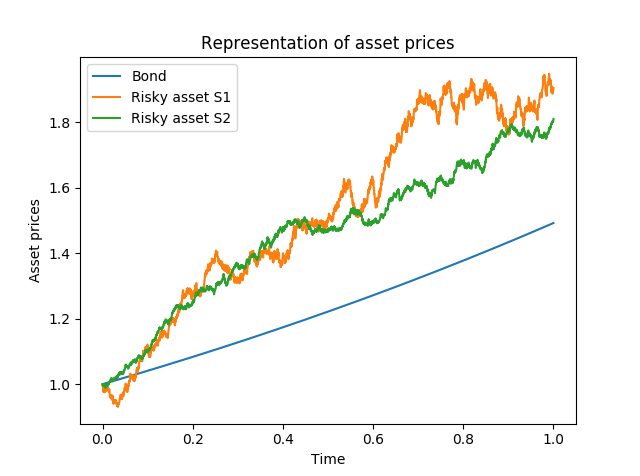
\includegraphics[width=0.7\textwidth]{images/market.png}
  \caption{Marché simulé}
\end{figure} 
\frametitle{Marché}
\end{frame}

\begin{frame}
\begin{figure}[H]
  \centering
    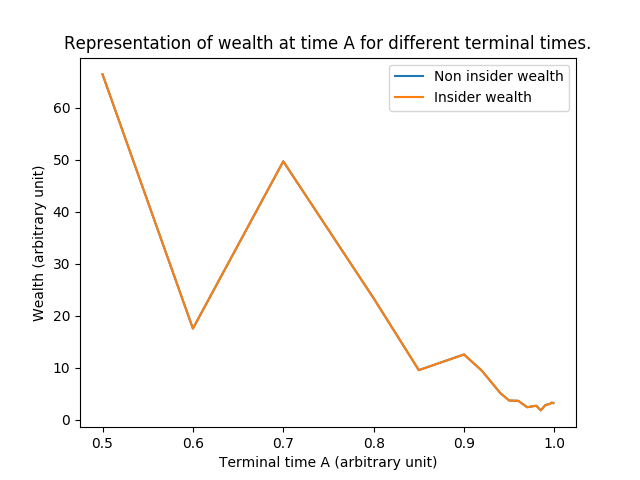
\includegraphics[width=0.7\textwidth]{images/wealths.png}
  \caption{Richesse des agents}
\end{figure} 
\frametitle{Richesses}
\end{frame}

\begin{frame}
\begin{figure}[H]
  \centering
    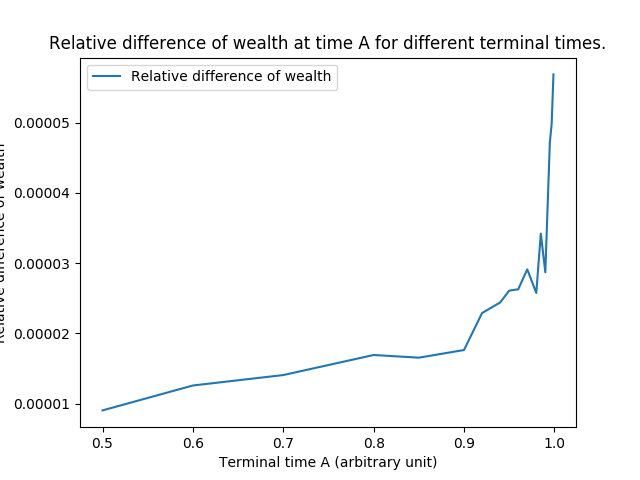
\includegraphics[width=0.7\textwidth]{images/relative_difference.png}
  \caption{Écart relatif des richesses}
\end{figure} 
\frametitle{Richesses}
\end{frame}

\section{Conclusion}
\begin{frame}
\begin{itemize}
	\item Compréhension générale du raisonnement de l'article.
	\item Implémentation informatique des formules dans un cas particulier.
\end{itemize}
\frametitle{Résumé}
\end{frame}

\begin{frame}
Approfondissement théorique : 
\begin{itemize}
	\item Cas plus réaliste : "bonds" de valeur dans le marché.
	\item Études de cas particuliers.
	\item ...
\end{itemize}
\frametitle{Perspectives du projet}
\end{frame}

\begin{frame}
\end{frame} % to enforce entries in the table of contents
\end{document}
